\documentclass[a4paper, 12pt, spanish]{article}

\usepackage[left=2.3cm, right= 1.8cm, top=2.5cm, bottom=2.2cm]{geometry}
\usepackage[es-tabla]{babel}
\usepackage{float}
\usepackage{tabto}
\usepackage{inconsolata}
\usepackage{graphicx}
\usepackage{wrapfig}
\usepackage{enumitem}
\usepackage{fancyhdr}
\usepackage{amsmath}
\usepackage{mathrsfs}
\usepackage{mathtools, nccmath}
\usepackage{index}
\usepackage{listings}
\usepackage{pdflscape}
\usepackage{multicol}
\usepackage{tikz}
\usepackage{marginnote}
\usepackage[format=plain,
            labelfont={it,bf},
            textfont=it, justification = centerlast]{caption}
\usetikzlibrary{calc,patterns,arrows,shapes.arrows,intersections, decorations.pathmorphing}
\usepackage[hidelinks, pdftex]{hyperref}
\usepackage[nameinlink]{cleveref}
\usepackage{subfig}
\usepackage{booktabs}
\usepackage{multirow}
\setlength{\columnsep}{1cm}
%\setlength{\columnseprule}{0.5pt}

\newcommand{\rot}{\nabla\times}

\crefname{table}{tabla}{tablas}
\Crefname{table}{Tabla}{Tablas}
\begin{document}
\pagestyle{fancy}\setcounter{page}{1}
\pagestyle{headings}
\begin{center}
\LARGE{\textbf{Propiedades Térmicas: Prácticas}} \rule{.9\textwidth}{.05cm}
\end{center}
\begin{flushright}
Alberto Peinador Veiga,\\
Universidad de Sevilla,\\
\Today
\end{flushright}

\begin{multicols}{2}
\section{Práctica 1: ciclo de histéresis.}
En la \Cref{fig:t} se representan los resultados de campo eléctrico y polarización con respecto al tiempo.
En ellos se ve como en todos los casos el campo eléctrico se mantiene independiente de la temperatura. La polarización si que tiene un respuesta diferente según la temperatura.\\
A temperatura baja la forma de la curva es muy similar a la del campo eléctrico. Se podría decir que son proporcionales, lo que concuerda con un régimen paraeléctrico. A temperaturas mayores, la polarización aumenta rápidamente en tiempos en los que el campo eléctrico es bajo hasta que llega a saturar. En el punto intermedio (\texttt{C6.DAT}) se puede percibir una combinación de ambas curvas.

\begin{figure}[H]
    \centering
    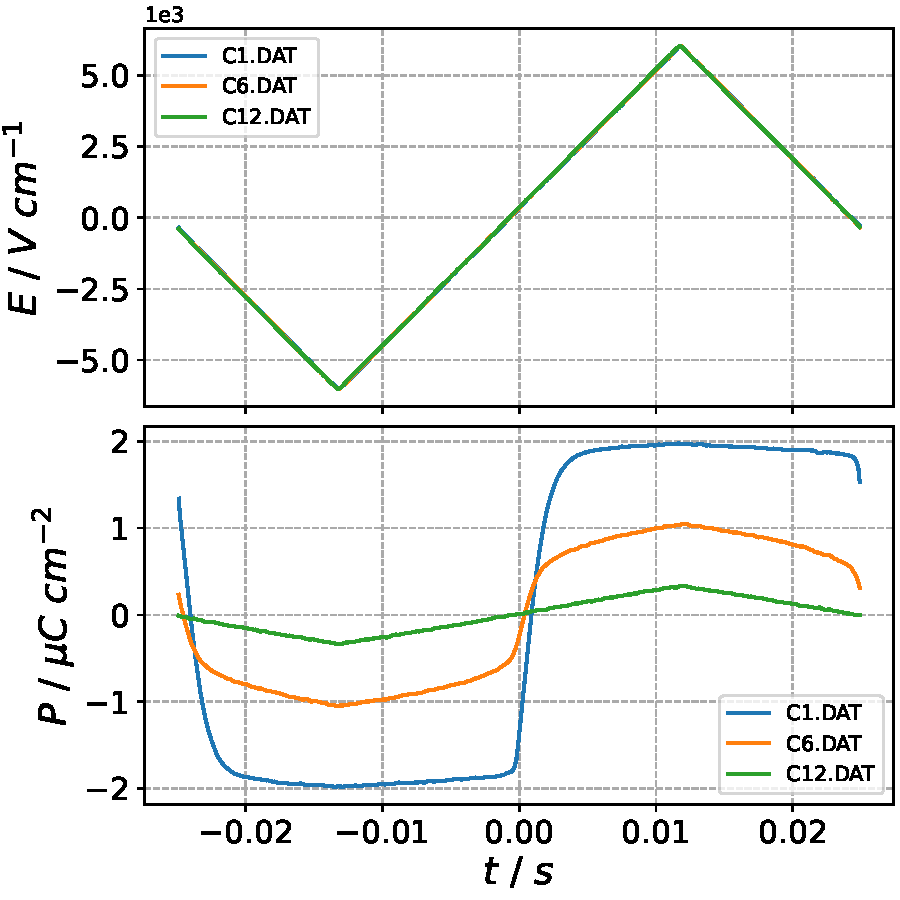
\includegraphics[width = \linewidth]{/Users/albertopeinador/Desktop/Master/termicas/E-t.pdf}
    \caption{Campo eléctrico y polarización como función del tiempo a distintas temperaturas.}\label{fig:t}
\end{figure}
La polarización remanente es la polarización cuando el campo eléctrico es nulo, mientras que el campo coercitivo es el campo eléctrico al que se anula la polarización. Para obtener estos parámetros se busca en los datos estos puntos, o en su defecto los más cercanos.\\
También se han tomado datos en ambas regiones: campo coercitivo y polarización remanente en ambos sentidos. 
\begin{table}[H]
    \centering
    \caption{Valores de $P_r$ y $E_c$ recogidos tanto para el TGS como para LATGS, calculados tomando la media entre los tres puntos más cercanos. Los valores se presentan en con las mismas unidades que en la \Cref{fig:t} y la temperatura en Kelvin.}\label{tab:Pr_ej1}
    \begin{tabular}{ccccc}\toprule
    Muestra & Sentido & T &$P_r$ & $E_c$\\ \midrule
    \multirow{6}*{TGS}& \multirow{3}*{(+)} & $310$ & $1.826$ & $799.3$\\
                        &                   &$318.6$ & $0.535$ & $558.9$\\
                        &                   &$324.6$ & $0.011$ & $149.2$\\ \cline{2-5}
                        & \multirow{3}*{(-)} & $310$ & $-1.813$ & $-814.7$\\
                        &                   &$318.6$ & $-0.522$ & $-554.7$\\
                        &                   &$324.6$ & $-0.004$ & $-153.2$\\ \midrule
    \multirow{2}*{LATGS} & (+) &$310$& $1.454$& $818.6$\\
    & (-) &$310$&$-1.105$&$-1213.2$\\ \bottomrule     
    \end{tabular}
\end{table}
Los valores para el TGS se representan en la \Cref{fig:param1}, junto a ellas se representa también el cuadrado de la polarización remanente, que según la teoría de Landau debería ser lineal con la temperatura. Sin embargo, como se ve con tan solo estos 3 puntos, parece no serlo en este rango de temperaturas. Si hacemos este mismo análisis con todas las curvas proporcionadas (\Cref{fig:Pr2}) se comprueba que sí existe un régimen lineal.
\begin{figure}[H]
    \centering
    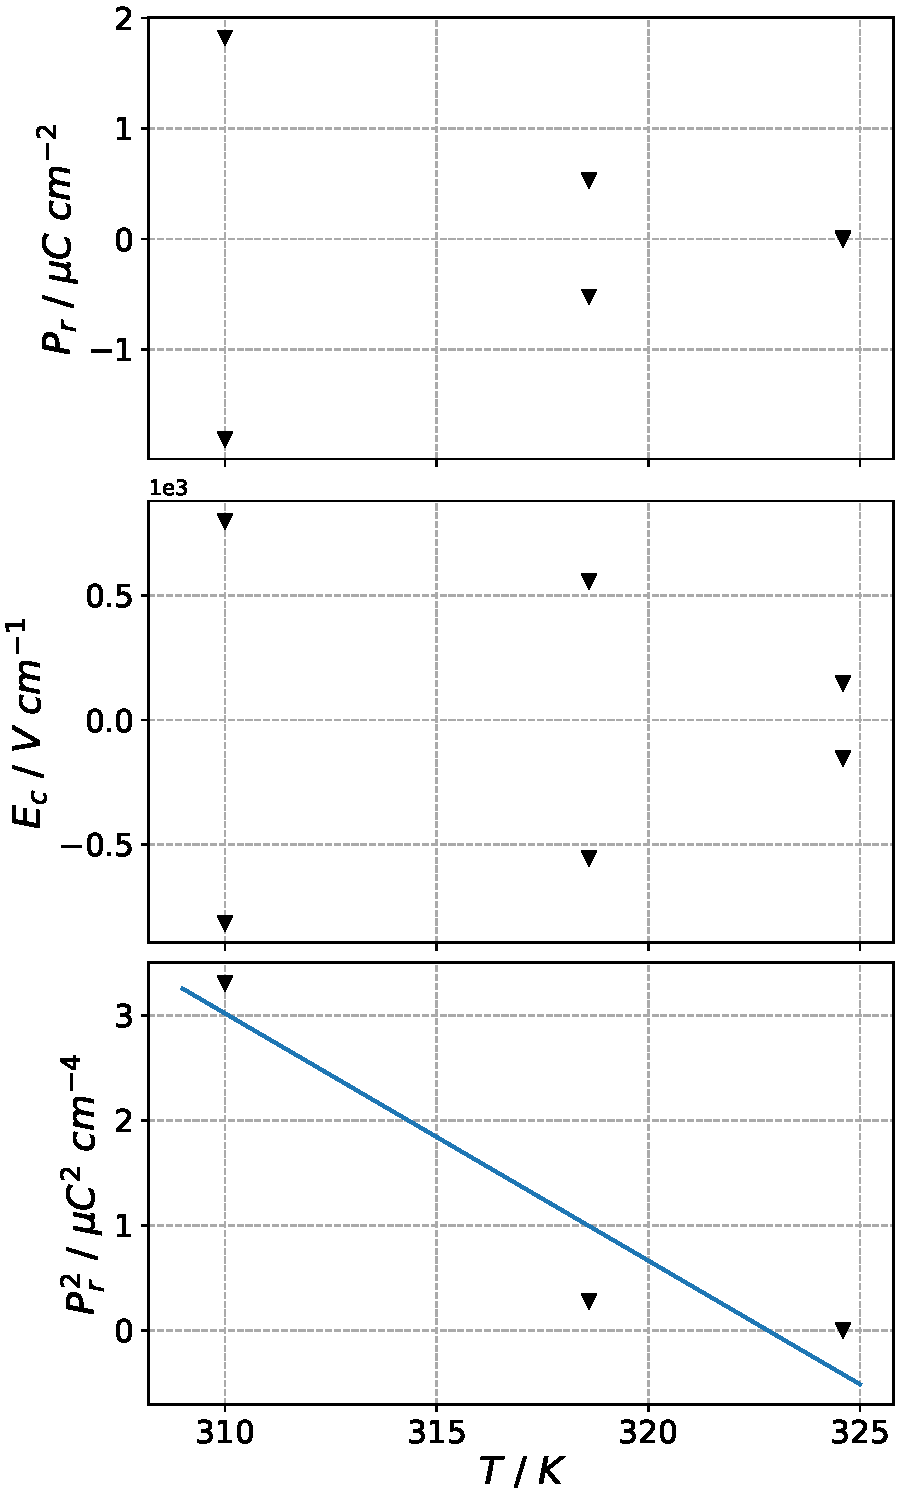
\includegraphics[width = \linewidth]{/Users/albertopeinador/Desktop/Master/termicas/Pr.pdf}
    \caption{Polarización remanente (a) y campo coercitivo (b) frente a temperatura así como una comprobación de la teoría de Landau (c)}\label{fig:param1}
\end{figure}
Tanto en las \Cref{fig:param1,fig:Pr2} se aprecia la disminución de tanto el campo coercitivo como de la polarización remanente. Es decir, los ciclos se estrechan (reducción de campo coercitivo) y desaparece la polarización remanente, pasando entonces de un ciclo de histéresis a, esencialmente, una recta. La respuesta lineal se asocia a una fase paraeléctrica y la pérdida gradual de $P_r$ y $E_c$ parece indecar que se trata de una transición de segundo orden, ya que el ciclo no desaparece abruptamente.
\begin{figure}[H]
    \centering
    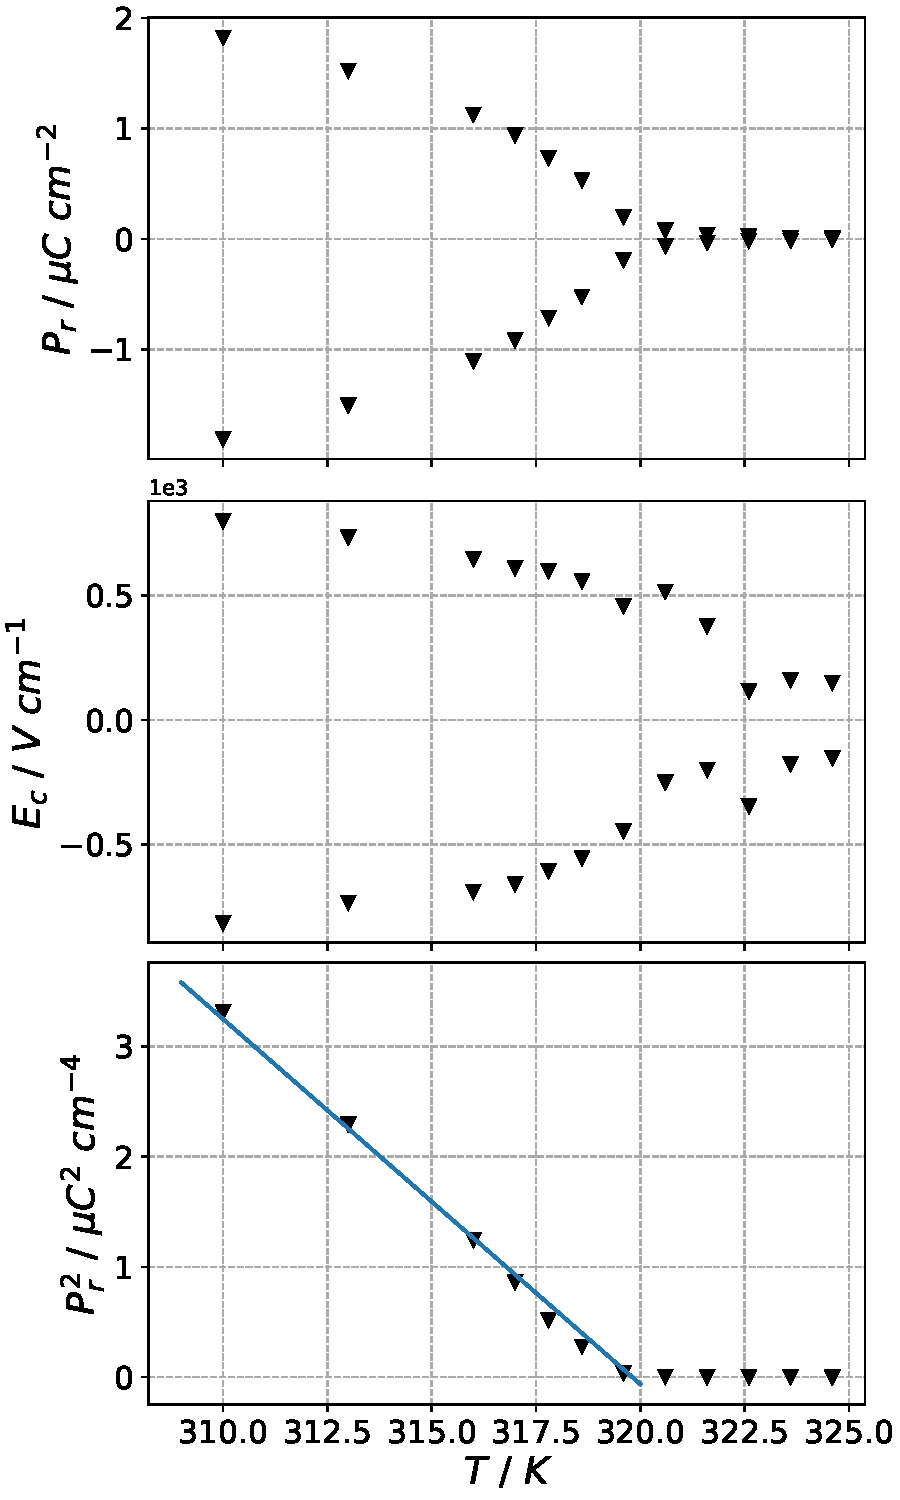
\includegraphics[width = \linewidth]{/Users/albertopeinador/Desktop/Master/termicas/Pr_2.pdf}
    \caption{Mismo análisis que el de la \Cref{fig:param1} incluyendo todas las temperaturas}\label{fig:Pr2}
\end{figure}

Retomando los resultados resumidos en la \Cref{tab:Pr_ej1}, se observa que los ciclos del TGS están bastante centrados, ya que los valores son bastante independientes del sentido en que se midan.\\
Por otra banda, el LATGS sí presenta un desplazamiento, al menos, en el campo eléctrico. Este desplazamiento es de $\Delta E = 394.6\ V\ cm^{-1}$ hacia el sentido negativo del campo. Este desplazamiento se explica como un campo eléctrico interno generado en el material.\\
En cuanto al desplazamiento vertical del ciclo no es correcto calcularlo con la polarización remanente recogida en la \Cref{tab:Pr_ej1}, puesto que $\Delta E$ provoca una disminución (en valor absoluto) de la polarización remanente negativa. Para obtener este desplazamiento, lo más correcto es utilizar la polarización de saturación. Los valores de polarización de saturación se obtienen buscando el máximo y el mínimo del ciclo; los valores obtenidos han sido: $P_{sat,\ (-)} = -1.755\ \mu C\ cm^{-2}$ y $P_{sat,\ (+)} = 1.577\ \mu C\ cm^{-2}$. Resultando un desplazamiento de $\Delta P = -0.178\ \mu C\ cm^{-2}$.

\section{Práctica 2: constante dieléctrica.}
\subsection*{Constante dieléctrica}
En la \Cref{fig:eps} se representa la constante dieléctrica calculada con la \cref{eq:eps}. Se perciben diferencias notables entre las dos muestras. El TGS puro presenta un pico muy pronunciado en la temperatura de Curie ($T_c\approx 322\ K$), por simple inspección parece que esta temperatura se desplaza, buscando el máximo de ambas curvas, se encuentra una diferencia de aproximadamente $0.3\ K$.\\
Las diferencias principales que se encuentran entre las dos curvas son el ancho e intensidad del pico. El LATGS presenta un pico mucho más ancho y un orden de magnitud más bajo que el de TGS. Este ancheamiento es útil en el diseño de sensores, ya que producirá una señal más estable en las proximidades del pico.

\begin{eqnarray}
    \varepsilon = \frac{C\ d}{\varepsilon_0\ S} \label{eq:eps}
\end{eqnarray}
\begin{figure}[H]
    \centering
    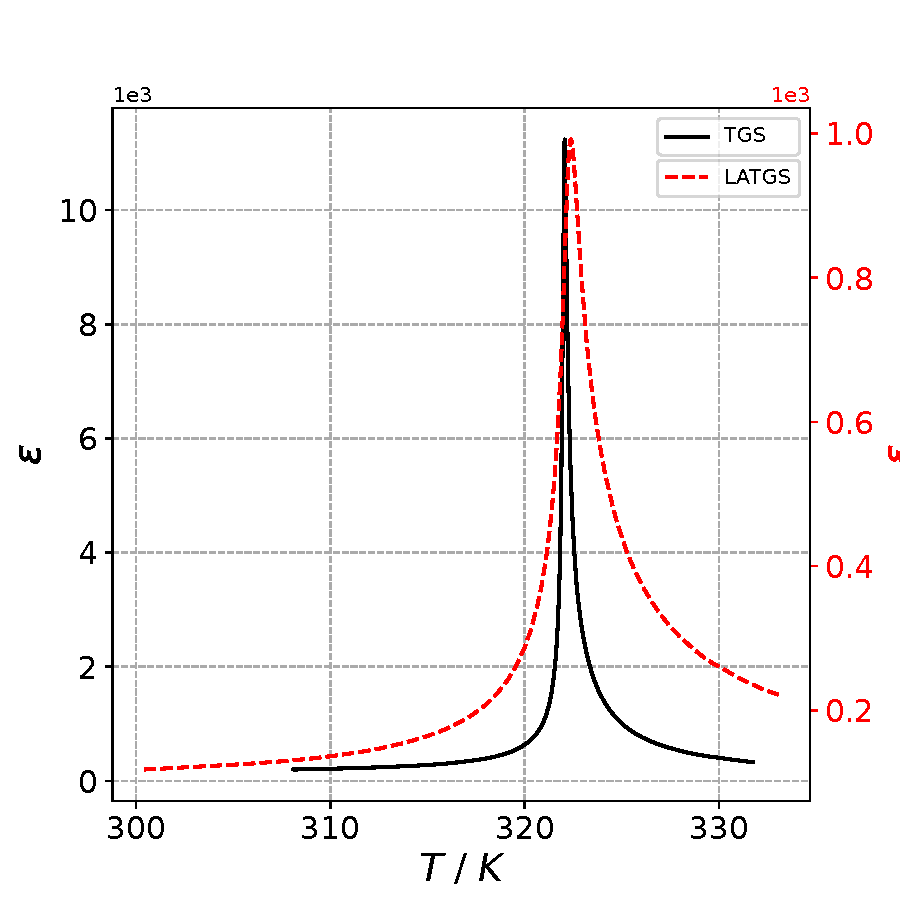
\includegraphics[width = \linewidth]{/Users/albertopeinador/Desktop/Master/termicas/ctedie.pdf}
    \caption{Constante dieléctrica de TGS (negro) y LATGS (rojo) con la escala reajustada.}\label{fig:eps}
\end{figure}
\subsection*{Ley de Curie-Weiss y teoría de Landau}
La ley de Curie-Weiss \cref{eq:cw} predice una relación lineal entre la inversa de la constante dieléctrica y la temperatura.
\begin{eqnarray}
    \frac{1}{\varepsilon} = \frac{T}{C_{CW}}-\frac{T_c}{C_{CW}}\label{eq:cw}
\end{eqnarray}
En la \Cref{fig:cw} se representa la inversa de $\varepsilon$ junto con un ajuste lineal por mínimos cuadrados que permite calcular la constante de Curie-Weiss ($C_{CW}$) y la temperatura de Curie ($T_c$)
\begin{figure}[H]
    \centering
    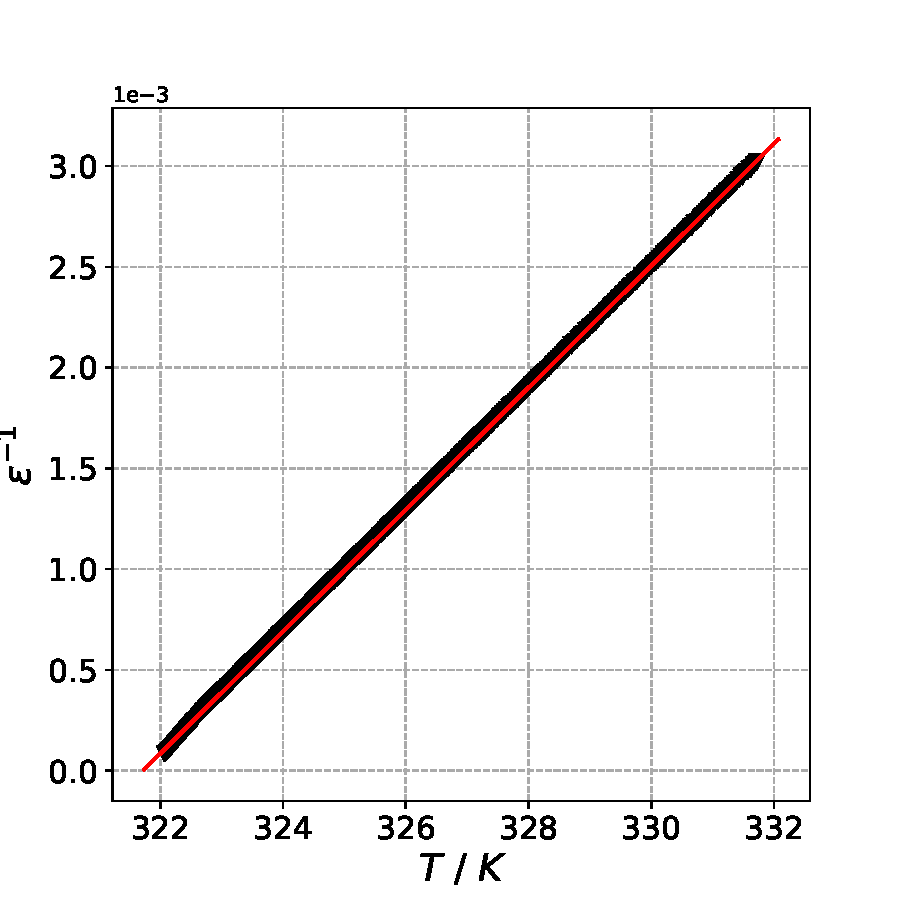
\includegraphics[width = \linewidth]{/Users/albertopeinador/Desktop/Master/termicas/cw.pdf}
    \caption{Comprobación de la ley de Curie-Weiss para la muestra de TGS.}\label{fig:cw}
\end{figure}

Por comparación con la \cref{eq:cw}, se calculan $C_{CW}$ y $T_c$ a partir de los parámetros de ajuste.\begin{eqnarray}
    C_{CW} = 3305.6\ K\\
    T_c = 321.7\ K
\end{eqnarray}
Por otro lado, la teoría de Landau predice una relación lineal también en el régimen ferroeléctrico ($T<T_c$). Donde la pendiente sería el doble de la pendiente de la \Cref{fig:cw} (en negativo). Haciendo el ajuste (\Cref{fig:l}) se comprueba que este no es el caso con nuestra muestra. Esta desviación puede deberse a efectos producidos por la formación de polidominios.
\begin{figure}[H]
    \centering
    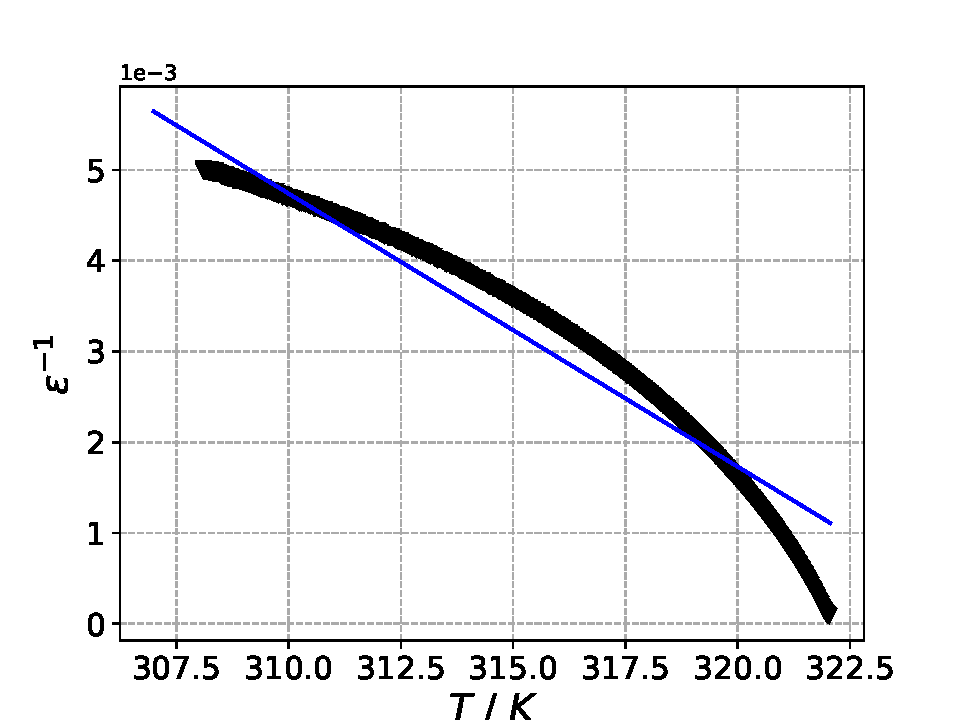
\includegraphics[width = \linewidth]{/Users/albertopeinador/Desktop/Master/termicas/l.pdf}
    \caption{Comprobación de la teoría de Landau para la muestra de TGS. Los puntos más alejados de $T_c$ sí parece que pudieran formar una recta, también en las proximidades muy cercanas a $T_c$. Estas dos regiones se ajustan en la \Cref{fig:l_2}}\label{fig:l}
\end{figure}
\begin{figure}[H]
    \centering
    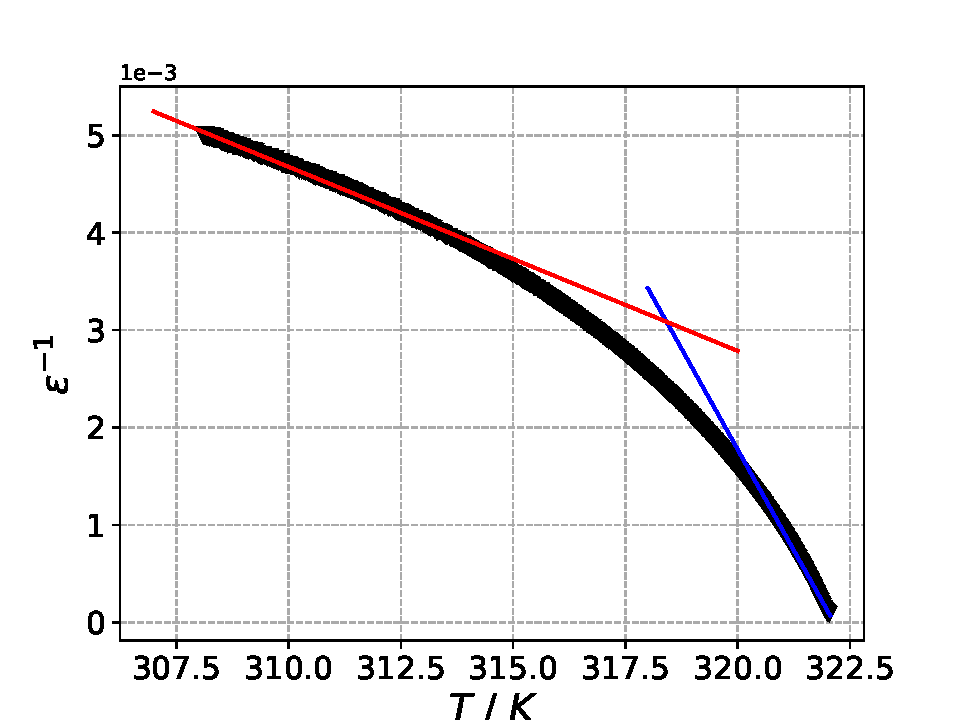
\includegraphics[width = \linewidth]{/Users/albertopeinador/Desktop/Master/termicas/l_2fit.pdf}
    \caption{Ajustes por zonas de la región ferroeléctrica. De la zona cercana a $T_c$ resulta una pendiente cercana al doble de la \Cref{fig:cw}, mientras que en la zona lejana la pendiente es menor que la de Curie Weiss.}\label{fig:l_2}
\end{figure}

\section{Práctica 3: coeficiente piroeléctrico}
\subsection*{Corriente piroeléctrica y polarización}
En primer lugar se representa la corriente piroeléctrica generada por la muestra frente a la temperatura(\Cref{fig:ip}).
\begin{figure}[H]
    \centering
    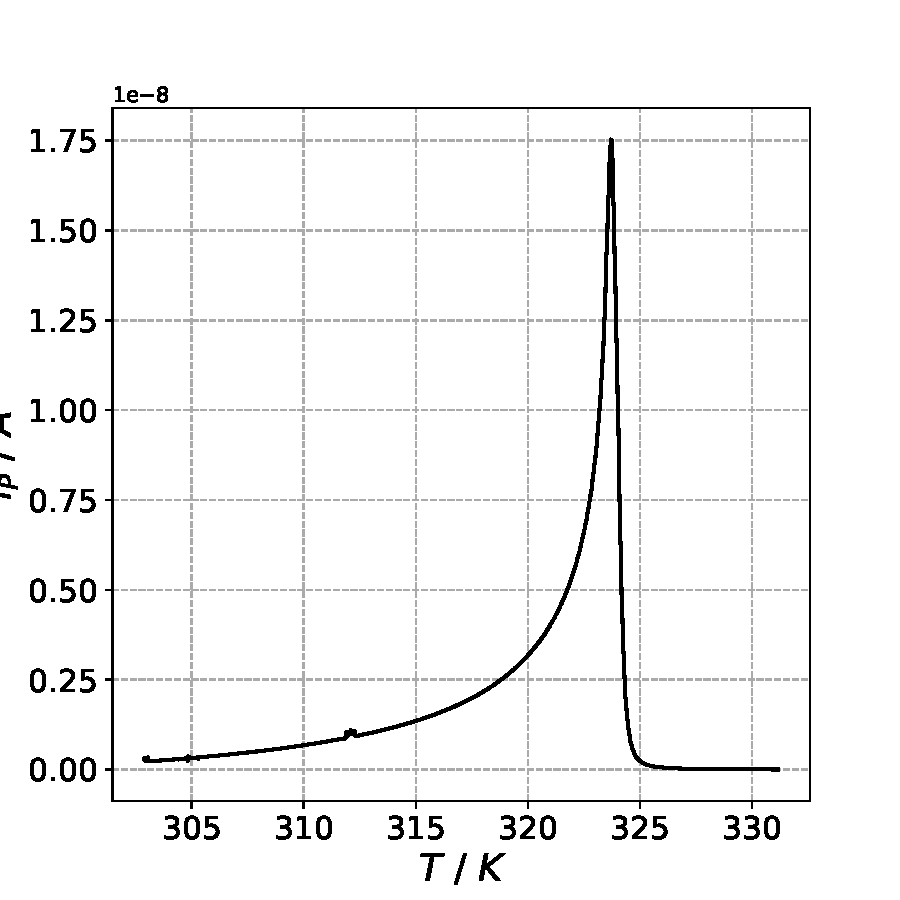
\includegraphics[width = \linewidth]{/Users/albertopeinador/Desktop/Master/termicas/ip.pdf}
    \caption{Corriente piroeléctrica generada frente a la temperatura.}\label{fig:ip}
\end{figure}
Con los datos proporcionados se calcula el coeficiente piroeléctrica ($\pi$) mediante la \cref{eq:pi}. Al integrar numéricamente en función a la temperatura (con el método de los trapecios), nos permite obtener los valores de polarización, representados en la \Cref{fig:pol}.
\begin{eqnarray}
    \pi = \frac{i_p}{r\ S}\label{eq:pi}
\end{eqnarray}

\begin{figure}[H]
    \centering
    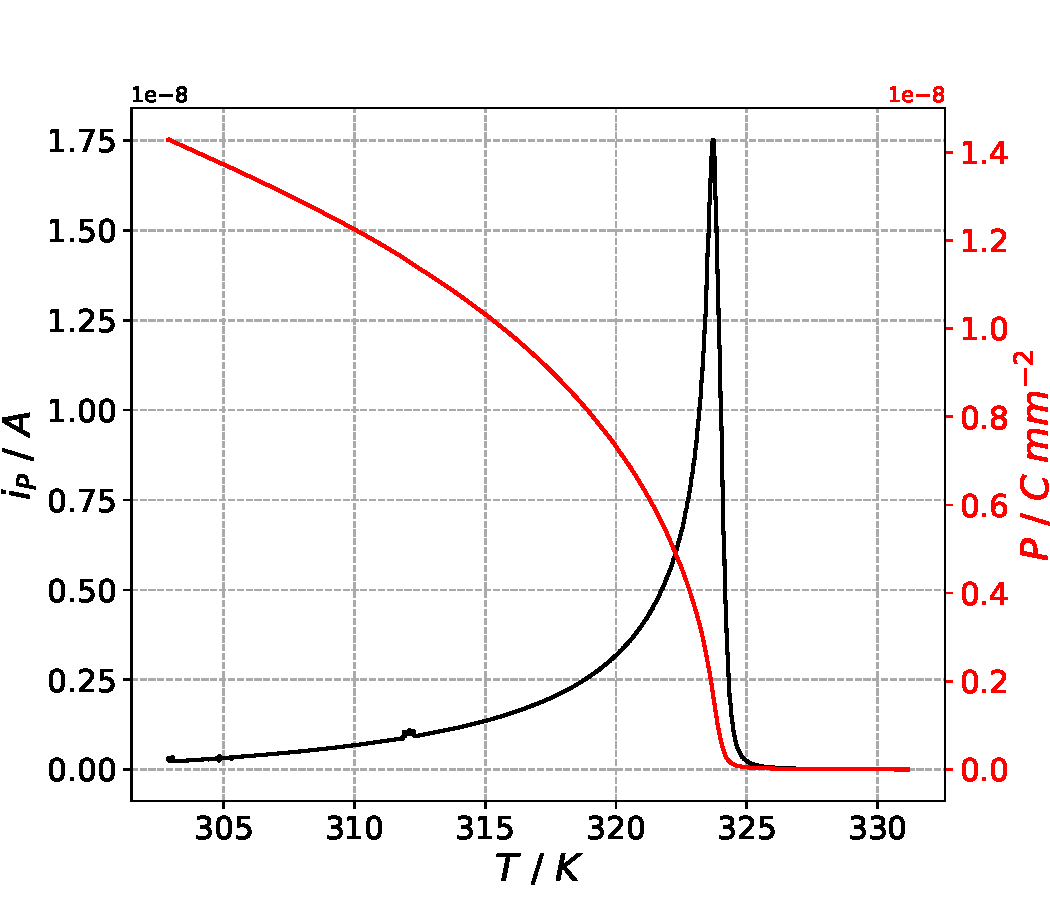
\includegraphics[width = \linewidth]{/Users/albertopeinador/Desktop/Master/termicas/P.pdf}
    \caption{Polarización calculada por integración del coeficiente piroeléctrico junto con la corriente piroeléctrica.}\label{fig:pol}
\end{figure}
\subsection*{Figura piroeléctrica de mérito}
%     ###################    (SUB)TABLES EXAMPLES      ###################


%\begin{table}[htpb]
%    \centering
%    \caption{Resumen de los picos observados en el espectro general.}
%    \subfloat[Fotoelectrones]{%
%        \begin{tabular}{ccc}
%			\toprule
%Elemento & Orbital & $E_B\ /\ eV$ \\ \midrule
%Na & 1s & 1070 \\
%Zn & 2p & 1020 \\
%Cu & 2p & 930 \\
%F & 1s & 683\\
%O & 1s & 531\\
%Ca & 2s & 438\\
%C&1s&284.6 \\ 
%Ar & 2p & 243\\
%Mo & 3d & 230\\
%Cu & 3s & 119\\
%Cu & 3p & 74\\
%\bottomrule
%        \end{tabular}
%        \label{tab:picos_ye}%
%    }
%    \qquad \ \qquad
%    \subfloat[Electrones Auger]{%
%        \begin{tabular}{ccc}
%            \toprule
%            Elemento & Transición & $K\ /\ eV$ \\ \midrule
%             Mo & NMV & 186 \\
%             C & KLL & 266\\
%             O & KLL & 489\\
%             F & KLL & 657\\
%             Zn & LMM & 989\\
%             Mg & KLL & 1179\\
%            \bottomrule
%        \end{tabular}
%        \label{tab:picos_auger}%
%    }
%    \label{tab:picos}
%\end{table}

%     ###################    (SUB)FIGURES EXAMPLES      ###################

%\begin{figure}[h!]
  %\centering
  %\subfloat[\label{fig:zona1A}]{%
  %  \includegraphics[width=0.49\linewidth]{Espectros/esctro_zona1}
  %}
  %\hfill
  %\subfloat[\label{fig:zona1B}]{%
  %  \includegraphics[width=0.49\linewidth]{Espectros/esctro_zona1_B}
  %}
  %\caption{Espectros con mayor resolución en la zona del pico de Zn 2p en energía cinética (a) y binding energy (b).}
%  \label{fig:zona1}
%\end{figure}


%\bibliographystyle{my_bibstyle}
%\bibliography{biblio.bib}



\end{multicols}
\end{document}
